\chapter{Experimentos} % ## 6. Experimentos

Como forma de testar o sistema desenvolvido, elaborou-se situações hipotéticas que se assemelhem às reais como forma de testar a eficiência do sistema. Para isso, utilizou-se como base os dados disponibilizados pelo coordenador do curso e pelo diretor do CCT. Em seguida, montou-se a estrutura de dados com a qual o sistema trabalhará analisando conflitos, e por fim, elaborou-se uma grade horária com base nos dados coletados.

\section{Aquisição dos dados} % ### 6.1. Aquisição dos dados

Como o acesso aos dados reais é restrito, vê-se necessário o uso de alternativas para que se possa validar os casos de uso do software desenvolvido.

Para se manter o mais próximo possível da realidade dos dados, utilizou-se os seguintes métodos como base os dados:

\begin{itemize}
  \item Disciplinas e requisitos: ementa de Ciência da Computação de 2015;
  \item Capacidades de salas e disciplinas ministradas por professores: pdf gerado pelo diretor do CCT quanto à oferta de salas;
  \item Alunos e progressão: dados disponibilizados pelo coordenador do Curso de computação;
  \item Preferências de alunos: formulário quantitativo.
\end{itemize}

% - Disciplinas e requisitos: ementa de Ciência da Computação de 2015;
% - Capacidades de salas e disciplinas ministradas por professores: pdf gerado pelo diretor do CCT quanto à oferta de salas;
% - Alunos e progressão: dados disponibilizados pelo coordenador do Curso de computação;
% - Preferências de alunos: formulário quantitativo.

Considerando as tabelas de dados necessárias para a criação de uma grade horária, utilizou-se do site \href{https://www.mockaroo.com/}{Mockaroo} para a geração de dados aleatórios que restam, sendo eles a preferência dos professores e as informações das disciplinas ministradas pelos professores não listados

Tendo os dados em mãos, resta então o uso prático do software para a alocação de turmas.

\section{Cenários} % ### 6.2. Cenários

Utilizando dos dados obtidos, elaborou-se então um cenário hipotético de criação de grade horária. Considerando assim a demanda de cada um dos alunos, a preferência de horários dos professores, a capacidade das salas e as disciplinas ministradas pelos professores.

Dispondo de todas essas informações e do software desenvolvido, foi possível então inicialmente distribuir as disciplinas em salas e horários segundo suas distribuições existentes nos semestres anteriores. Assim já podendo visualizar os conflitos que ocorreram neste período.

% A imagem abaixo apresenta um segmento de distribuição de disciplinas listadas pelo CCT e seus respectivos retornos visuais quanto aos conflitos encontrados:

% \begin{figure}[htbp]\centering
% \caption{\label{DistribuicaoInicial}Disposição inicial das disciplinas}
% 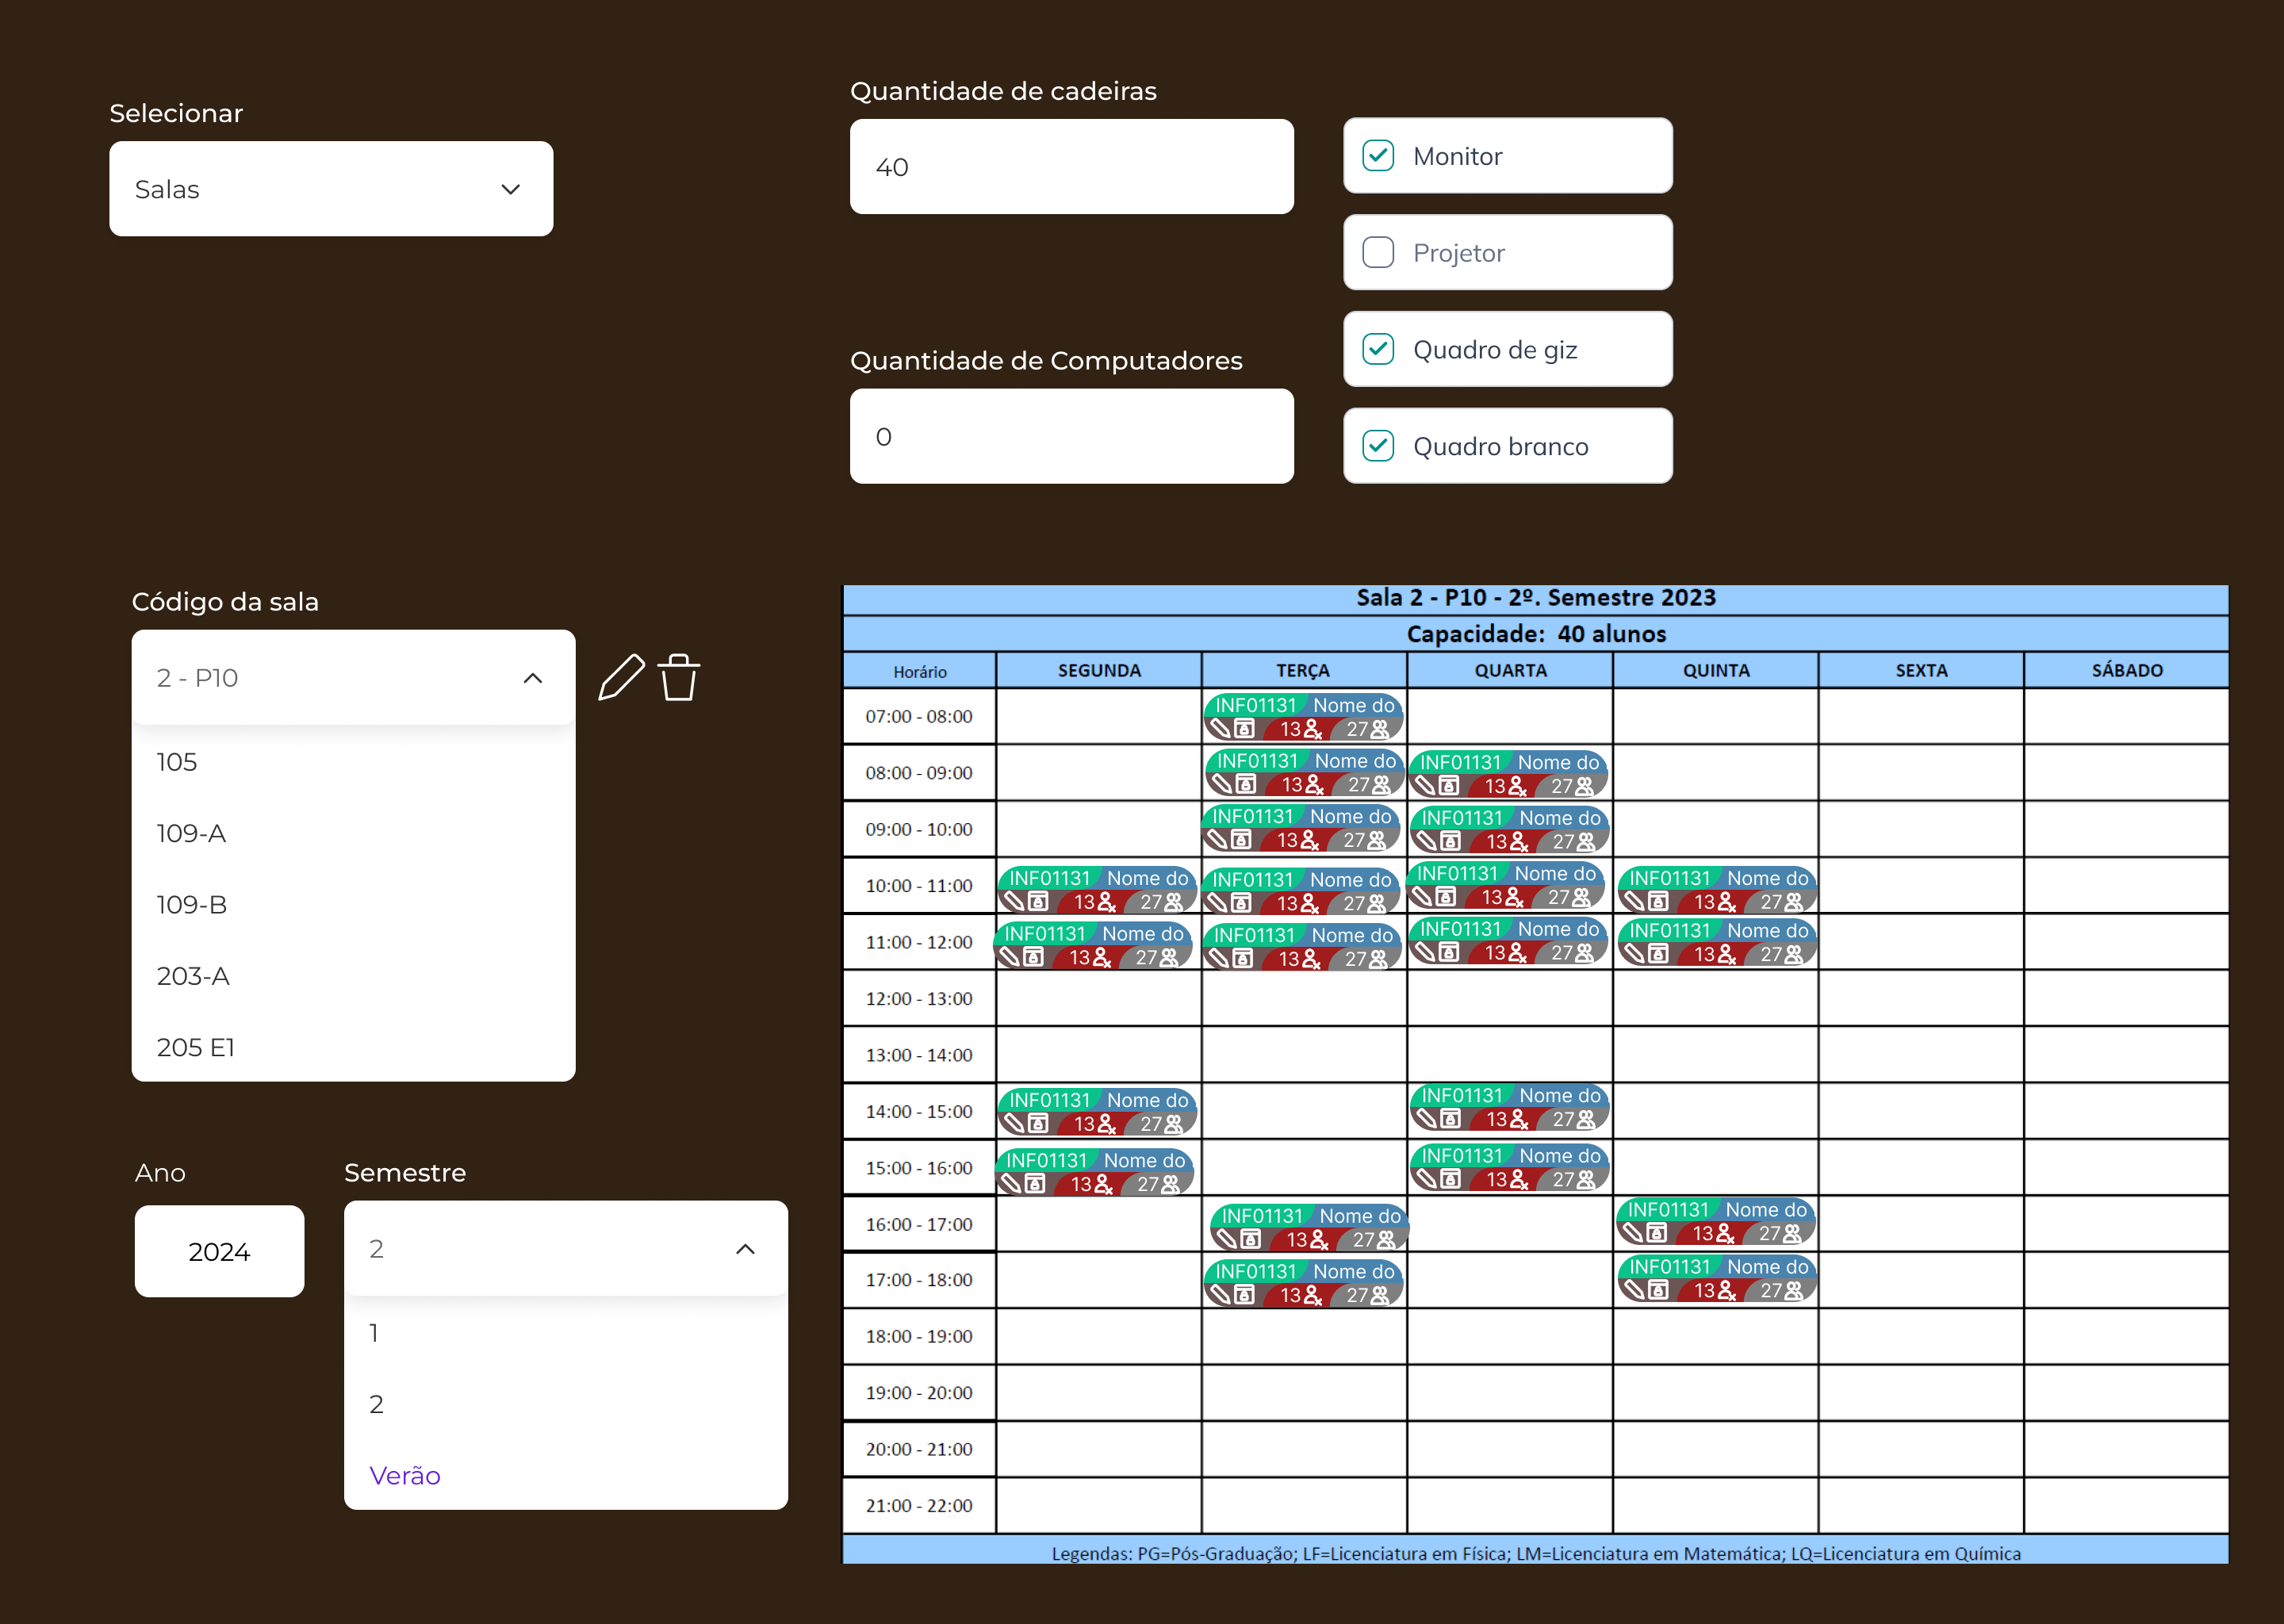
\includegraphics[scale=0.8]{files/img/Experimentos/SituacaoInicial.png}
% \legend{Fonte: o autor}
% \end{figure}    % Distribuição inicial das disciplinas
% ![Alt text](img/Experimentos/SituacaoInicial.png)

% Nessa imagem, vemos que algumas das turmas foram alocadas em salas que não possuem a capacidade necessária para a quantidade de alunos que demandam a disciplina. Além disso, vemos que algumas das turmas foram alocadas em horários que não condizem com a preferência dos professores.

% \begin{figure}[htbp]\centering
% \caption{\label{DistribuicaoAprimorada}Disposição aprimorada das disciplinas}
% 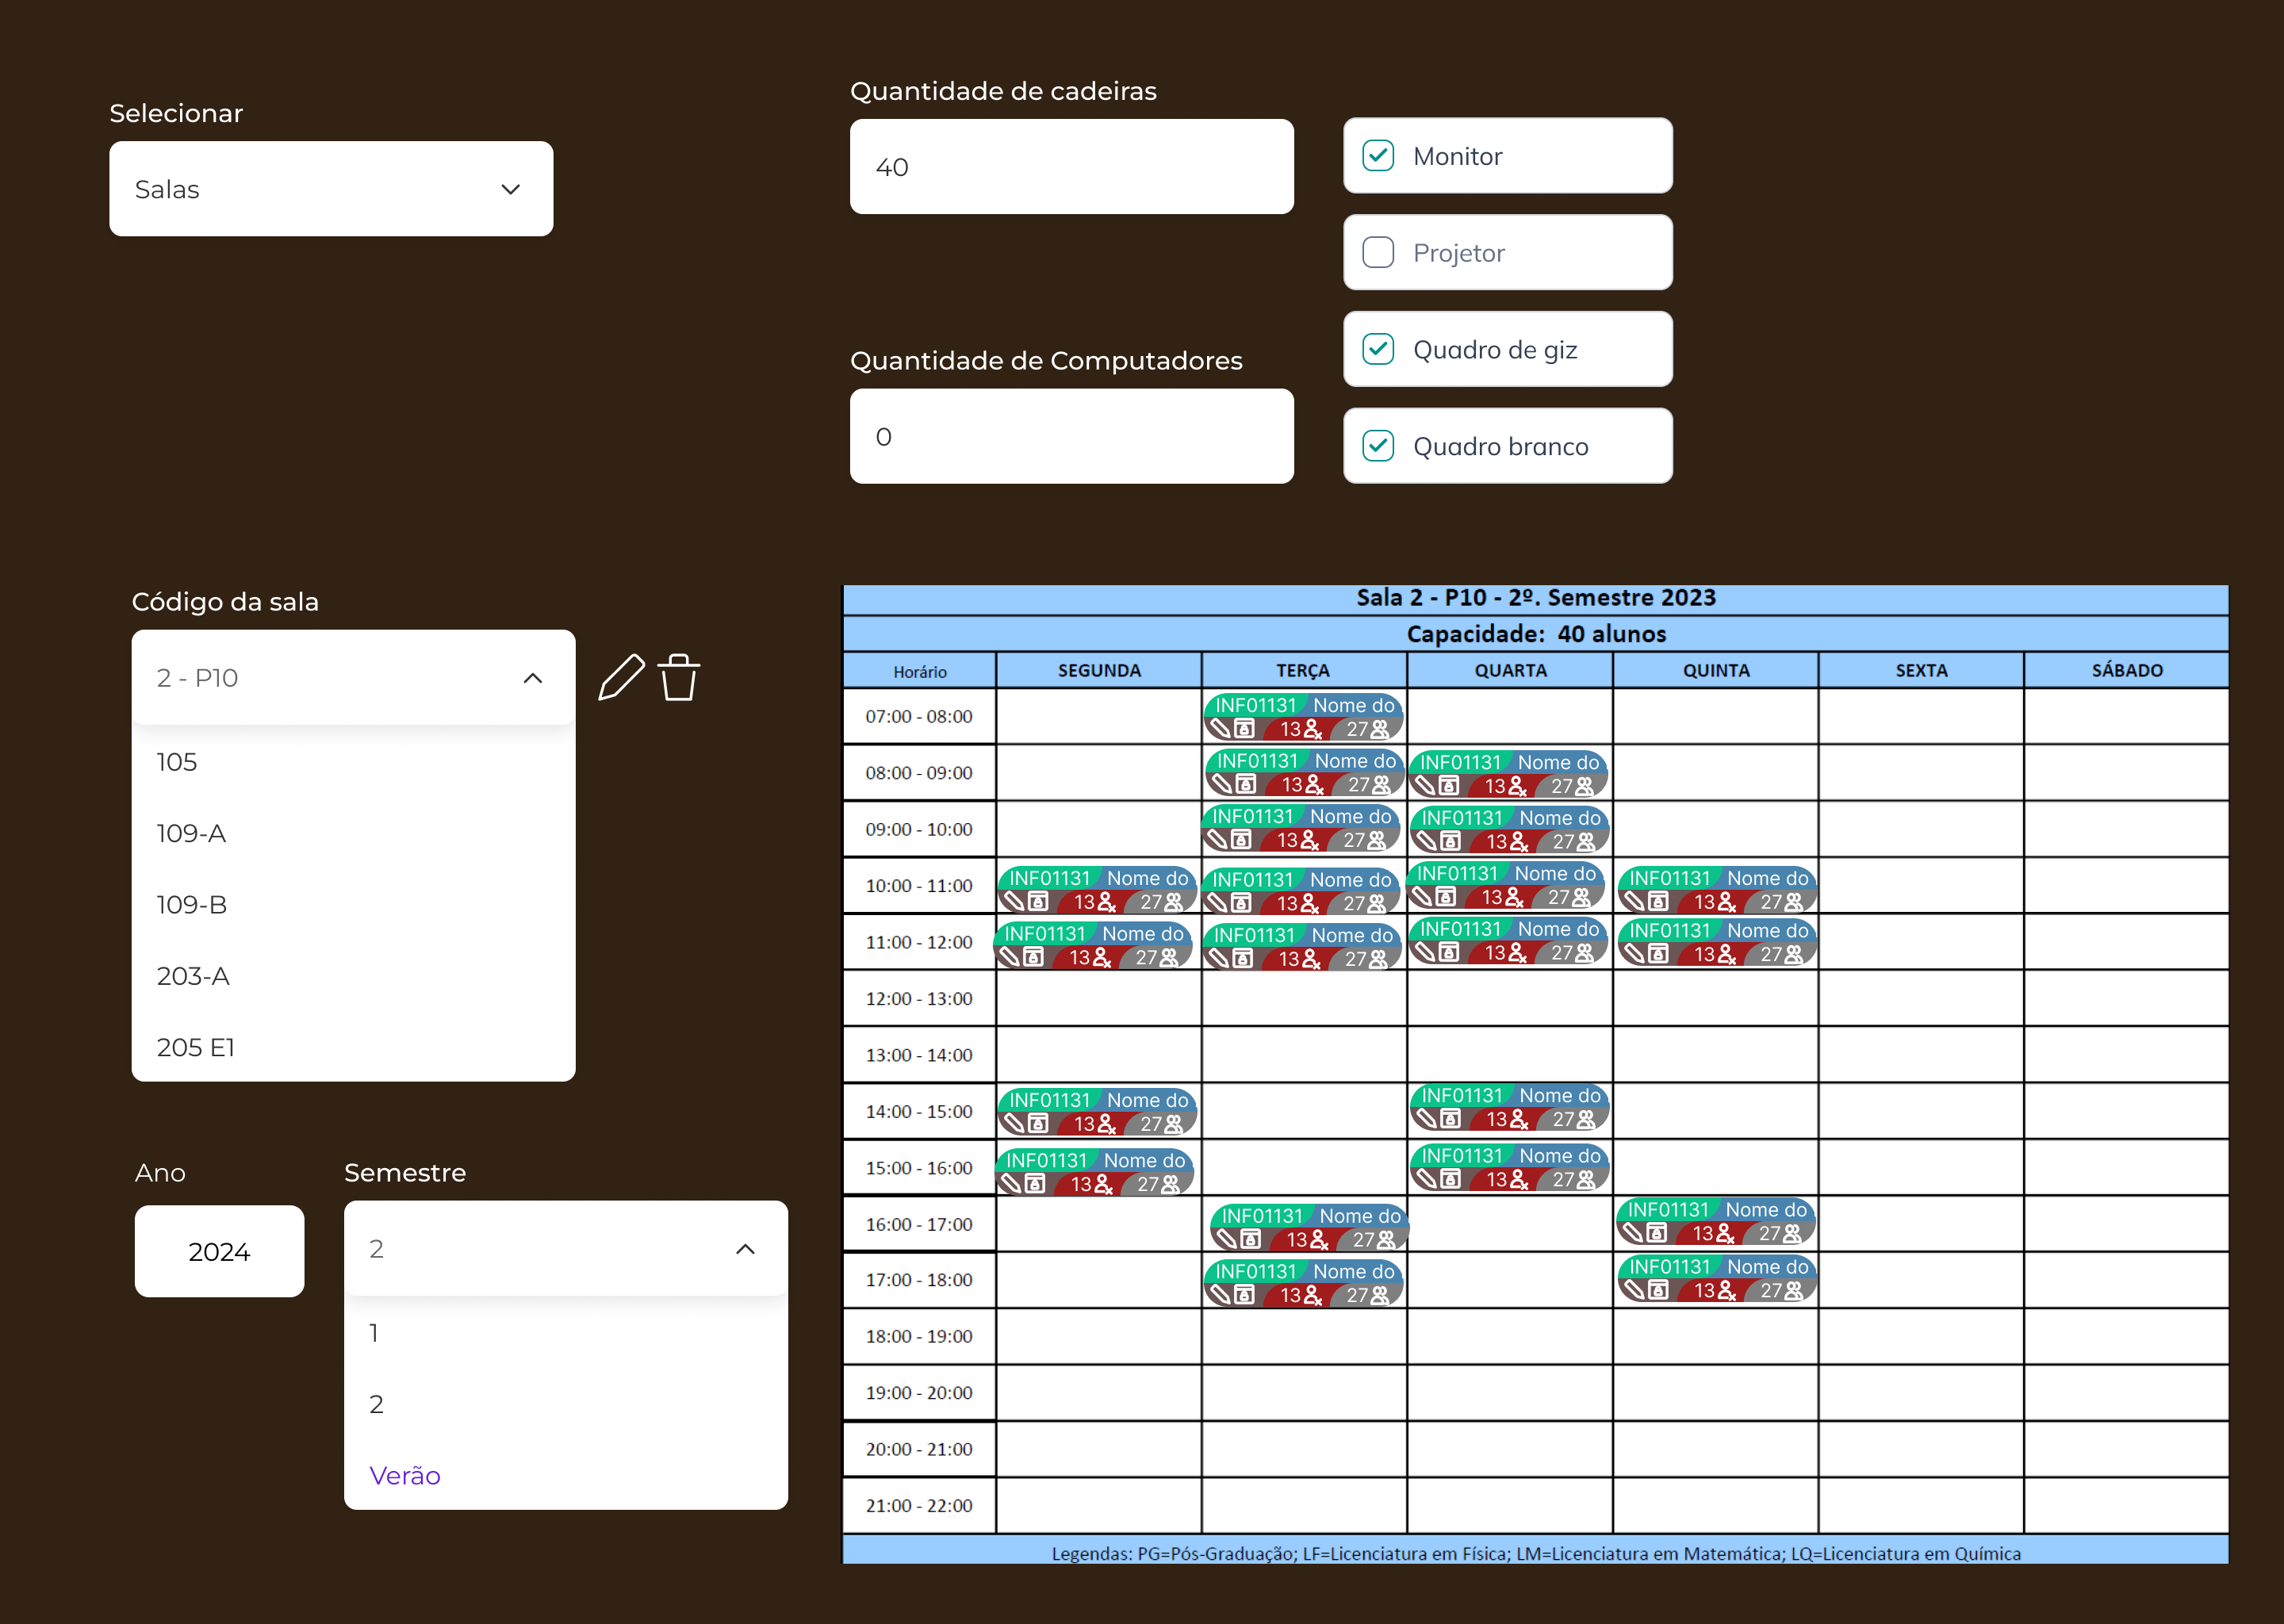
\includegraphics[scale=0.8]{files/img/Experimentos/Aprimoramento.png}
% \legend{Fonte: o autor}
% \end{figure}    % Distribuição aprimorada das disciplinas
% ![Alt text](img/Experimentos/Aprimoramento.png)

Com as alterações na tabela inicial de distribuição de disciplinas, foi possível obter uma grade horária com menos conflitos e que se aproxima mais da preferência dos professores.

